\subsection*{آ و پ}

فرم درختی یک روش مدل‌سازی است که برای بازی‌های با توالی زمانی مشخص و تصمیم‌های چندگانه استفاده می‌شود. در این روش، بازی به صورت یک درخت تصمیم‌گیری مدل‌سازی می‌شود. هر گره درخت نماینده یک وضعیت خاص از بازی است و هر یال به یک تصمیم انجام شده و یا عملیاتی که اجرا می‌شود متصل می‌شود. درخت پیمایش می‌شود تا به وضعیت نهایی بازی برسد و نتایج و پاداش‌های متناسب با هر حالت و تصمیم درخت در نظر گرفته می‌شوند. فرم درختی به ما اجازه می‌دهد تا تصمیمات و تأثیرات آن‌ها را به صورت سلسله مراتبی مدل‌سازی کنیم.


از طرفی، فرم نرمال یک روش مدل‌سازی است که برای بازی‌های با توالی زمانی نامعلوم یا همزمان استفاده می‌شود. در این روش، بازی به صورت یک جدول ساده یا نمودار مدل‌سازی می‌شود. در هر سطر از جدول، تمام بازیکنان تصمیمات خود را به صورت همزمان اعمال می‌کنند. هر بازیکن در ستونی از جدول قرار می‌گیرد و نتیجه هر حالت به طور مجزا در نظر گرفته می‌شود. فرم نرمال به ما اجازه می‌دهد تا تعامل‌های همزمان و ناسازگار را در بازی مدل‌سازی کنیم.


ابتدا می‌دانیم که حالت‌های آ و پ یکسان هستند وقتی همزمان تصمیم می‌گیرند A و B ، عملا مانند زمانی‌ست که فرض می‌کنیم انتخاب‌های همدیگر را نمی‌دانند.

استراتژی ز اکیدا مغلوب است و با توجه به بهترین انتخاب‌ها می‌بینیم که سپس ک انتخاب می‌شود در هر دو سمت پس داریم که تعادل زیربازی کامل، (ک و ک) است.

\begin{center}
	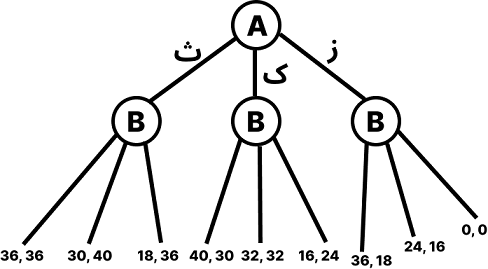
\includegraphics{Tree2}
\end{center}

\begin{center}
	\begin{tabular}{||c c c c||} 
		\hline
		$Z$ & $K$ & $S$ & $$ \\ [0.5ex] 
		\hline\hline
		$18 , 36$ & $30 , 40$ & $36 , 36$ & $S$ \\ 
		\hline
		$16 , 24$ & $32 , 32$ & $40 , 30$ & $K$ \\
		\hline
		$0 , 0$ & $24 , 16$ & $36 , 18$ & $Z$ \\
		\hline
	\end{tabular}
\end{center}


\subsection*{ب}

انتخاب‌های A و ‌B مشخص شده است و تعادل زیربازی کامل، (ز و ث) است.

\begin{center}
	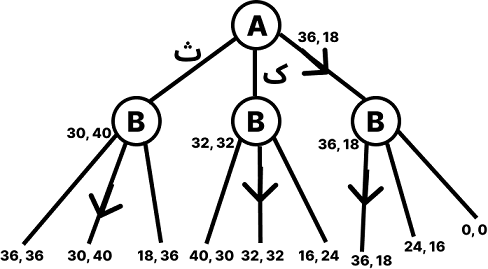
\includegraphics{Tree3}
\end{center}